\subsection{Clustering}
\label{sec:clustering}

We compared three clustering algorithms applied to the original
substitute vectors using many-to-one accuracy on the PTB24K.
Hierarchical agglomerative clustering with complete linkage (HAC)
starts with each instance in its own cluster and iteratively combines
the two closest groups (measured by their most distant points) at each
step \cite{manning2008introduction}.  K-medoids minimizes sum of
pairwise distances between each data-point to the exemplar at the
center of its cluster \cite{kaufman2005finding}.  Spectral
clustering\footnote{We used the implementation in
  \cite{chen2011parallel} with a symmetric sparse affinity matrix of
  550 nearest neighbors.} uses the eigenvalues of the graph Laplacian
$L=D^{-1/2} W D^{-1/2}$ to reduce the number of dimensions (similar to
Laplacian eigenmaps) and uses simple k-means clustering on the
resulting representation \cite{ng2002spectral}.  All three algorithms
accept the distance matrix based on the KL2 distance (see
Section~\ref{sec:dist}) as input.

\begin{figure}[h] \centering
  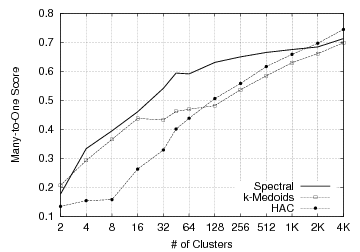
\includegraphics[width=0.6\textwidth]{clustering_graph_mono.png}
\caption{Many-to-one score for three clustering algorithms on the
  45-tag 24K word corpus.}
\label{fig:clustering}
\end{figure}

% #cluster kmedoid spectral hac
% 2          0.20795 0.17781 0.135762
% 4          0.29413 0.33439 0.155579
% 8          0.36615 0.39550 0.159076
% 16        0.43830 0.46116 0.263988
% 32        0.43318 0.54192 0.329850
% 45        0.46245 0.59413 0.401832
% 64        0.46965 0.59151 0.438843
% 128      0.48235 0.63106 0.506703
% 256      0.53709 0.65000 0.558659
% 512      0.58464 0.66520 0.616653
% 1024     0.62985 0.67523 0.658576
% 2048     0.66107 0.68414 0.696878
% 4096     0.69842 0.71286 0.744338


Figure~\ref{fig:clustering} plots the many-to-one score versus number
of clusters for the three algorithms on the PTB24K.  The many-to-one
score naturally increases as we approach the one cluster per word
limit, however we find the evolution of the curves informative.  At
the high end (more than 2000 clusters) HAC performs best with its
conservative clusters, but its performance degrades fast as we reduce
the number of clusters because it cannot reverse the accumulating
mistakes.  At the low end (less than 16 clusters) k-medoids and
spectral have similar performance.  However for the region of interest
(between 16 to 2000 clusters) spectral clustering is clearly superior
with \spectralResult \mto accuracy at 45 clusters.

We noted that the 45 cluster spectral clustering result assigned many
more tags to each word than the gold standard.  To apply
one-tag-per-word restriction we collapse the tag assignment of
spectral clustering by re-taging each word with its most frequent tag
in the original assignment (we break ties randomly).  Collapsing
improves the many-to-one accuracy by more than 10\% from
\spectralResult\% to \collapseResult\%.

In accord with the findings and results on the PTB24K, we perform
spectral clustering on the PTB by using the language model defined in
Section~\ref{sec:expset} together with the Manhattan similarity
metric\footnote{The new language model in Section~\ref{sec:expset}
  only calculates the top 100 substitutes and set the ones other than
  the top 100 to 0 which results in sparse substitute vectors.  As a
  results the new model is computationally more efficient than the one
  in this section and it is more appropriate for large datasets like
  the PTB.  KL2 is undefined on sparse vectors, therefore we use
  Manhattan which is the successor of KL2 on both the PTB24K and PTB.}
and achieve \spectralResultPTB \mto (\collapseResultPTB \vm) accuracy
which is comparable with the results on the PTB24.

%% Section~\ref{sec:dist} reveals that using the language model described
%% in Section~\cite{sec:lm}.  Using the top 100 substitutes results in
%% sparse substitute vectors on which KL2 is undefined.  However scores
%% of similarity metrics on PTB found to be in line with results on
%% PTB24K from Section~\ref{sec:dist}. Thus KL2's successor Manhattan
%% metric is chosen for spectral clustering.

%% Spectral clustering on 1M word data set scored ??\mto accuracy.  To
%% enforce one-tag-per-word assumption we assigned each word to its most
%% observed cluster which increased the \mto accuracy to ??.


% LocalWords:  PTB
